\section{Semi-Supervised Approaches}\label{sec:semi-supervised-approaches}

This chapter expands the scope of trade classification from the supervised setting to the semi-supervised setting and presents suitable extensions.

\subsection{Framing as a Semi-supervised Learning Problem}\label{sec:problem-framing-2}

The supervised approaches depend on the availability of the trade initiator as the true label. Yet, obtaining the label is often restricted to the rare cases, where the trade initiator is provided by the exchange or to subsets of trades where the initiator can be inferred through matching procedures (cp. \cref{sec:trade-initiator}). This may bias the selection. Unlabeled trades, though, are abundant and can help improve the generalization performance of the classifier. This concern is addressed by semi-supervised methods.

Semi-supervised methods leverage partially-labeled data by learning an algorithm on unlabeled instances alongside true labels \autocite[][2]{chapelleSemisupervisedLearning2006}. They are centered around the semi-supervised assumption of smoothness, which states that if two samples say $\mathbf{x}_{1}$ and $\mathbf{x}_{2}$ are nearby in a high-density region, their class labels $y_{1}$ and $y_{2}$ should also be similar. Vice versa, if data points are separated by a low-density region, their labels may be different \autocite[][5]{chapelleSemisupervisedLearning2006}.

\begin{figure}[!h]
    \centering
    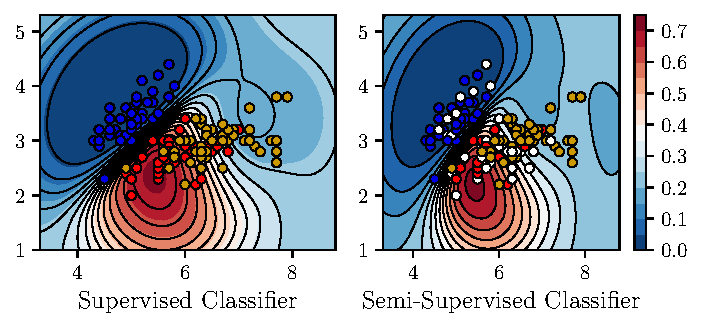
\includegraphics[width=0.8\linewidth]{decision-boundary-semi-supervised.pdf}
    \caption[Decision Boundary of Supervised and Semi-supervised Classifiers]{Decision boundary of a supervised and semi-supervised classifier. The supervised classifier is trained entirely on labeled data. The semi-supervised classifier uses both labeled and unlabeled instances to determine the decision boundary. Predicted class probabilities of \mycircle{viz-red} are visualized as a contour. Here, the unlabeled datapoints, drawn as \mycircle{viz-white}, lead to more confident predictions and a stretched class.}
    \label{fig:supervised-semi-supervised}
\end{figure}

Applied to trade classification, with semi-supervised methods we implicitly assume that trades with similar features, such as a common trade price and quotes, conform to the same class. The purpose of unlabeled trades is to help efficiently determine the boundary around regions of neighboring trades resulting in improved generalization performance. A visualization of decision boundaries of (semi-)supervised classifiers is given in \cref{fig:supervised-semi-supervised}.

The semi-supervised setting requires extending our notation from \cref{sec:problem-framing}, by distinguishing between labeled and unlabeled instances. Like before, $\mathcal{D}=\left\{\left(\mathbf{x}_i, y_i\right)\right\}_{i=1}^N$ denotes all labeled trades. Unlabeled data points are stored in a separate set $\mathcal{U} = \left\{\mathbf{x}_i\right\}_{i=1}^{K}$. We subsequently discuss and select two approaches for semi-supervised trade classification.

\subsection{Selection of Approaches}\label{sec:selection-of-approaches-1}

Our goal is to extend \glspl{GBRT} and Transformers for the semi-supervised setting to make use of the abundant, unlabeled trade data. We are aimed to make minimally intrusive changes to maintain a fair comparison with the supervised counterparts. We find self-training for gradient boosting and pre-training of Transformers suitable for training on labeled and unlabeled trades, as our subsequent discussion derives.

\textbf{Gradient Boosting}

The success of supervised gradient boosting led to the development of gradient boosting for the semi-supervised setting. An early work of \textcite[][555--556]{dalche-bucSemisupervisedMarginBoost2001} explores replacing supervised weak learners, i.e., regression trees, with semi-supervised weak learners, i.e., mixture models and minimizes a loss function over labeled and unlabeled instances. Another line of research, including \textcites[][290--291]{bennettExploitingUnlabeledData2002}[][2003--2004]{mallapragadaSemiBoostBoostingSemiSupervised2009}, retain supervised weak learners to generate pseudo labels of unlabeled instances per iteration. True labeled and pseudo-labeled data is then used in fitting weak learners of subsequent iterations. Approaches differ regarding the selection criterion of the pseudo-labeled instances. Both lines of work, however, require changes to the boosting procedure or the base learners.

An alternative is to pair gradient boosting with self-training. Self-training is a wrapper algorithm around a supervised classifier, that incorporates its most-confident predictions of unlabeled instances into the training procedure \autocite[][190]{yarowskyUnsupervisedWordSense1995}. In contrast to previous methods, pseudo labels are generated exclusively from the fully-fledged ensemble, which is grown multiple times at a higher computational cost. Being a model-agnostic wrapper, it does not change the classifier and ensures maximum comparability. This, together with the widespread adoption in the literature, makes it a compelling choice for semi-supervised trade classification.

\textbf{Transformer}

Whilst Transformers could be combined with self-training, a more promising approach is to pre-train Transformers on unlabeled data, and then fine-tune the network on the remaining labeled instances. Various studies report unanimously performance improvements from pre-training tabular Transformers, including \textcites[][8]{somepalliSaintImprovedNeural2021}[][7--8]{huangTabTransformerTabularData2020}.

Until now we assumed the parameters e.g., weights and biases, of the Transformer to be initialized randomly. The joint goal of pre-training objectives is to initialize a neural network with weights that capture expressive representations of the input and thereby improve generalization performance over a random initialization when fine-tuning on a specific task \autocite[][636]{erhanWhyDoesUnsupervised}. The training is now decomposed into two stages: in the first stage the model is trained with respect to the pre-training objective to obtain the parameter estimates on unlabeled instances, and in the second stage the Transformer is initialized with the parameters and then finetuned on the labeled dataset. Particularly beneficial, general embeddings can be learned during pre-training, even if the true label, i.e., the trade initiator, is unknown or its definition varies between tasks.

Pre-training objectives for tabular data differ vastly in their methodology and are often directly adapted from other domains including \gls{MLM} \autocite[][4174]{devlinBERTPretrainingDeep2019}, \gls{RTD} \autocite[][2--3]{clarkElectraPretrainingText2020}, or contrastive learning \autocite[][1598]{chenSimpleFrameworkContrastive2020}.
As such, \textcite[][7]{huangTabTransformerTabularData2020} adapt \gls{MLM}, whereby features are randomly masked and the objective is to reconstruct the original input. Pre-training by \gls{RTD} aims to identify randomly replaced features and recover a binary mask used for replacement \autocite[][7]{huangTabTransformerTabularData2020}. \textcites[][3--4]{bahriSCARFSelfsupervisedContrastive2022}[][11036--11037]{yoonVIMEExtendingSuccess2020} reconstruct both the binary feature mask and the original input simultaneously. \textcite[][3]{somepalliSaintImprovedNeural2021} alter the methodology of \textcite[][11036--11037]{yoonVIMEExtendingSuccess2020} through a contrastive loss function.

With a multitude of methods, tested on different datasets and neural architectures, a fair comparison between pre-training methods is tedious. Yet, \textcite[][2-3]{rubachevRevisitingPretrainingObjectives2022} provide guidance in selecting objectives. Among the pre-training objectives that they benchmark, the \gls{RTD} objective was among the best-performing approaches. The \gls{RTD} objective is easy to optimize, unsupervised, and leaves the model architecture unaltered, which makes \gls{RTD} a compelling choice for pre-training on unlabeled data.

The next chapter covers self-training in detail.

\subsection{Gradient Boosted Trees With Self-Training}\label{sec:extensions-to-gradient-boosted-trees}

Self-training is a wrapper algorithm around a probabilistic classifier, that incorporates its predictions of unlabeled instances as pseudo labels \autocite[][190]{yarowskyUnsupervisedWordSense1995}.

Initially, a base classifier is fitted on the labeled data points in a supervised manner. The classifier then assigns labels, so-called pseudo labels, to unlabeled instances. A subset of unlabeled instances with high-confidence predictions is selected, removed from the unlabeled dataset, and added to the pseudo-labeled data dataset. A new classifier is then retrained on the labeled and pseudo-labeled instances \autocite[][190--192]{yarowskyUnsupervisedWordSense1995}. The process is repeated for several iterations until an abortion criterion applies, such as the maximum number of iterations is exhausted or when no unlabeled instances are left to label.

Recall from our discussion on \glspl{GBRT} in \cref{sec:gradient-boosting-procedure} that we optimized for the cross-entropy loss on the training set. When coupled with self-training in each training iteration the classifier $F$ now jointly minimizes the loss over the labeled samples $\mathcal{D}$ and the pseudo-labeled samples $\not{\mathcal{U}}$:
\begin{equation}
    \frac{1}{\left|\mathcal{D}\right|} \sum_{(\mathbf{x}, y) \in \mathcal{D}} L(F(\mathbf{x}), y)+\frac{\epsilon}{\left|\not{\mathcal{U}}\right|} \sum_{(\mathbf{x}, \tilde{y}) \in \not{\mathcal{U}}} L(F(\mathbf{x}), \tilde{y})+\lambda\|F\|^2,
\end{equation}
where $\epsilon$ is a hyperparameter to control the impact of the pseudo-labeled data, $\tilde{y}$ is the pseudo-labeled instance, and $\lambda$ weights the regularization term \autocite[][4]{aminiSelfTrainingSurvey2023}.

In every iteration, only unlabeled instances are added to the training set, for which the predicted class probability exceeds a confidence threshold. This approach has implications, as highlighted by \textcite[][32427]{chenDebiasedSelfTrainingSemiSupervised2022}. The threshold becomes an important hyperparameter in controlling that no noisy labels are added to the training set, but a restriction to highly-confidence samples may lead to a data bias and over-confidence in the prediction. Self-training is prone to a confirmation bias, as confident but wrong pseudo labels are erroneously incorporated into the training set, which in effect leads to a propagation of errors in the subsequent training rounds.

At the same time, self-training puts a high emphasis on the correctness of the probability estimates in the base classifier. This is problematic for decision trees, known to produce poor probability estimates, as probabilities are derived from the class frequency in the leaf node containing few samples \autocite[][357--358]{tanhaSemisupervisedSelftrainingDecision2017}. However, as gradient boosting directly optimizes for the cross-entropy loss, the problem found for its ensemble member no longer occurs.

Independent of the base classifier, self-training increases computational cost, as training is repeated over several iterations on a growing training set \autocite[][3841]{zophRethinkingPretrainingSelftraining2020}. Despite these limitations, the potentially improved decision boundary outweighs the concerns.

\subsection{Transformers With Pre-Training}\label{sec:extensions-to-transformer}

\gls{RTD} is a pre-training objective proposed by \textcite[][2--3]{clarkElectraPretrainingText2020} for the use in language models. The core idea is to randomly replace tokens with plausible alternatives and learn a binary classifier to distinguish between original and replaced tokens. Intuitionally, the random replacement forces the model to learn generalizable representations of the input, rather than memorizing the co-occurrence of certain tokens. Additionally, surprising the model with random tokens strengthens its ability to incorporate contextual information.

\begin{figure}[ht]
    \centering
    {\renewcommand\normalsize{\small}
        \normalsize
        \input{./Graphs/random-token-replacement.pdf_tex}}
    \caption[Replaced Token Detection]{Replaced Token Detection. Visualization inspired by \textcite[][3]{clarkElectraPretrainingText2020}.}
    \label{fig:random-token-replacement}
\end{figure}

Their approach uses two neural networks, namely the generator and the discriminator, typically implemented as Transformers, as visualized in \cref{fig:random-token-replacement}.  The generator is responsible for generating replacement tokens and receives an input sequence, i.e., a sentence, that has been intentionally masked out. It learns to predict the original token of the now-masked token through tokens in the bidirectional context (cp. \cref{sec:attention}). For masking, an additional $\mathtt{[MASK]}$ token is introduced, which extends the vocabulary (cp. \cref{sec:token-embeddings}). Separately for each token, the final hidden state of the masked token is fed through a softmax activation to obtain the predicted probability distribution of the masked token, and the cross entropy loss is used to compare against the true distribution. By replacing the masked token with a token from the generator distribution, convincing replacements now take place for some of the original inputs \autocite[][2--3]{clarkElectraPretrainingText2020}.

The discriminator then receives the corrupted input sequence and is trained to distinguish between original and replaced tokens originating from the generator. The output is a binary mask to be compared against the mask initially used for masking tokens in the generator \autocite[][2--3]{clarkElectraPretrainingText2020}.

Applied to tabular datasets, \gls{RTD} transfers to randomly replacing feature values in $\mathbf{x}_{i}$ instead of sequences. The objective is now to predict a binary mask $\mathbf{m}_{i}\in \{0,1\}^{M}$ corresponding to $\mathbf{x}_{i}$, indicating which features, or entries in $\mathbf{x}_{i}$, have been replaced. Previous adaptions for tabular data, e.g., \textcite[][3]{huangTabTransformerTabularData2020}, simplify the replacement strategy by sampling replacement values directly from the feature, which alleviates the need for a generator network and requires less compute. Since the replacement is done on a feature-per-feature basis, the replaced token is \emph{per se} harder to detect.

For tabular data, the random replacement of feature values also strengthens the model's ability to incorporate a combination of features, rather than a single or few features based on their absolute value, which would facilitate overfitting.

In summary, \gls{RTD} can help to learn expressive representations of the input, even if the true label is unavailable. Given previous research, we expect pre-training \gls{RTD} to improve the performance of the FT-Transformer and match or exceed the of the \gls{GBRT}.